\begin{figure}[H]
    \centering
    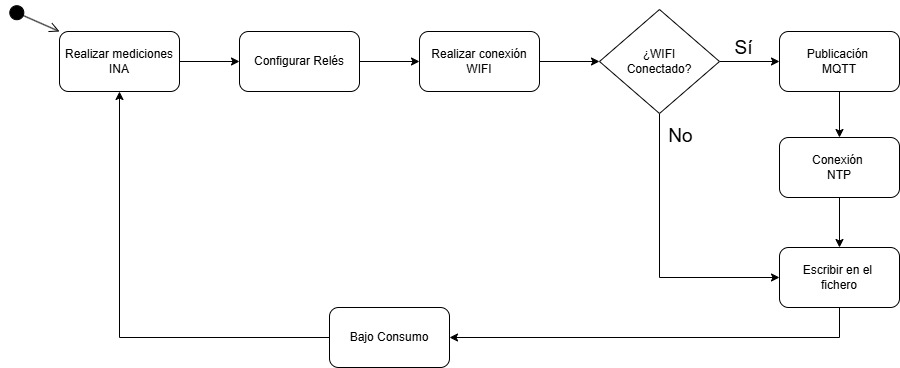
\includegraphics[width=0.95\textwidth]{images/3-software/3-3-programaprincipal/DiagramaDeFlujoPOWER.jpg}
    \caption{Diagrama de flujo Programa Principal}
    \label{fig:3-3-1-DiagramaFlujo}
\end{figure}

Para la implementación del programa principal, también se han desarrollado dos funciones adicionales que se encargan de intentar la conexión WIFI y configurar los relés del sistema. A continuación, se explican dichas funciones:

\begin{itemize}
    \item Función \texttt{setup\_wifi()}: esta función es la encargada de la conexión WIFI del sistema. Se intentará la conexión un número determinado de intentos, definidos en la variable \texttt{WIFI\_TRIES}. Esta función no recibe ningún parámetro y tampoco devuelve nada.
    \begin{lstlisting}[captionpos=b, caption={Definición función setup\_wifi}, language=c++]
        static void setup_wifi();
    \end{lstlisting}
    La secuencia de ejecución de esta función es la siguiente:
    \begin{enumerate}
        \item Muestra por serial un mensaje con la red WIFI a la que se intenta la conexión.
        \item Intenta realizar la conexión a la red WIFI con las credenciales almacenadas en las variables \texttt{ssid} y \texttt{password}. Estas variables almacenan el nombre de la red WIFI y su correspondiente contraseña, respectivamente.
        \item Se intenta realizar la conexión un número finito de intentos indicados en la variable

        \texttt{WIFI\_TRIES}. El tiempo de espera entre intentos de conexión es de 500ms.
        \item En caso de que la conexión haya sido satisfactoria, el sistema mostrará por serial un mensaje al usuario indicando que la conexión WIFI se ha realizado correctamente. En este mensaje se mostrará el nombre de la red a la que se ha realizado la conexión y la dirección IP de nuestro dispositivo ESP8266.
        \item Por otra parte, en caso de que el sistema no haya sido capaz de conectarse a la red WIFI indicada, se mostrará un mensaje de error por serial indicando al usuario la conexión fallida.
    \end{enumerate}
    \begin{lstlisting}[captionpos=b, caption={Desarrollo función setup\_wifi}, language=c++]
        static void setup_wifi() {
            delay(10);
            Serial.print("[WIFI] Intentando conectar a " ssid);
            WiFi.begin(ssid, password);
            for (int i = 0; i < WIFI_TRIES && WiFi.status() != WL_CONNECTED; i++) {
                delay(500);
                Serial.print(".");
                i++;
            }
            if (WiFi.status() == WL_CONNECTED) {
                PRINT_DEBUG("[WIFI] Conectado a la red WiFi " ssid " con IP: ");
                PRINT_DEBUG(WiFi.localIP());
            } else {
                PRINT_DEBUG("[WIFI] No se ha podido conectar a la red WiFi");
            }
        }
    \end{lstlisting}
    \item Función \texttt{setRelays}: esta función es la encargada de configurar los relés del sistema en función de los valores medidos por los sensores y de los valores almacenados en las variables \texttt{SOLAR\_THRESH} y \texttt{BAT\_THRESH}. Esta función recibe como parámetro un puntero a la vabiable \texttt{telemetry}, la cual almacena las medidas obtenidas por los diferentes sensores y no devuelve nada.
    \begin{lstlisting}[captionpos=b, caption={Definición función setRelays}, language=c++]
        static void setRelays(telemetry_t *telemetry);
    \end{lstlisting}
    Esta función se compone de tres casos para las diferentes posibilidades de funcionamiento del sistema. Estas opciones son las siguientes:
    \begin{itemize}
        \item VSolar $>$ \texttt{SOLAR\_THRESH}: esta posibilidad se refleja cuando la tensión medida en el panel solar es mayor al valor del \texttt{threshold} solar, almacenado en dicha variable. Esto quiere decir que la energía aportada por el panel solar es suficiente para asegurar el correcto funcionamiento y cargar de forma adecuada tanto la batería de backup como las otras dos baterías de carga. En este caso, ambos relés están en la posición que hemos denominado \texttt{LOW}, conectando el panel solar y la batería de backup al resto del sistema.
        \item VBatbu $>$ \texttt{BAT\_THRESH}: en caso de que la tensión medida en el panel solar no sea suficiente para alimentar el circuito completo, se comprobará si la energía almacenada en la batería de backup es suficiente. Para ello, se compara la tensión medida en dicha batería con su respectivo \texttt{threshold}, almacenado en la variable \texttt{BAT\_THRESH}. En caso de que dicha tensión medida sea mayor, quiere decir que es suficiente para asegurar el correcto funcionamiento del sistema y la carga correcta de las otra dos batería. Para este caso, los relés conmutan a la posición denominada \texttt{HIGH}, la cual desconecta el panel solar del sistema y conecta la batería de backup al camino de alimentación del sistema.
        \item Por último, en caso de que ni la energía del panel solar ni la de la batería de backup sean suficientes para alimentar el circuito y cargar las dos baterías, se entiende que no hay manera de asegurar el correcto funcionamientod el sistema, por lo que los relés volveran a la posición inicial \texttt{LOW} pero, debido a que no hay alimentación suficiente, el sistema de apagará. El sistema permanecerá en este estado hasta que el panel solar vuelva a su funcionamiento nominal y pueda aportar la cantidad de energía suficiente para volver al comportamiento predeterminado del sistema, cargando tanto la batería de backup como las otras 2 baterías de carga.
    \end{itemize}
    \begin{lstlisting}[captionpos=b, caption={Desarrollo función setRelays}, language=c++]
        static void setRelays(telemetry_t *telemetry){
            if (telemetry->VSolar > SOLAR_THRESH) {
                PRINT_DEBUG("[RELAY] Panel solar activo");

                digitalWrite(RELAY_SW_IN,LOW);
                digitalWrite(RELAY_SW_OUT,LOW);
            } else if (telemetry->VBatbu > BAT_THRESH){
                PRINT_DEBUG("[RELAY] Bateria backup activa");

                digitalWrite(RELAY_SW_IN,HIGH);
                digitalWrite(RELAY_SW_OUT,HIGH);
            } else {
                PRINT_DEBUG("[RELAY] Activando proteccion sobredescarga. Se detendra el sistema");

                digitalWrite(RELAY_SW_IN,LOW);
                digitalWrite(RELAY_SW_OUT,LOW);
            }
        }
    \end{lstlisting}
\end{itemize}
